\documentclass[11pt,preprint, authoryear]{elsarticle}

\usepackage{lmodern}
%%%% My spacing
\usepackage{setspace}
\setstretch{1.2}
\DeclareMathSizes{12}{14}{10}{10}

% Wrap around which gives all figures included the [H] command, or places it "here". This can be tedious to code in Rmarkdown.
\usepackage{float}
\let\origfigure\figure
\let\endorigfigure\endfigure
\renewenvironment{figure}[1][2] {
    \expandafter\origfigure\expandafter[H]
} {
    \endorigfigure
}

\let\origtable\table
\let\endorigtable\endtable
\renewenvironment{table}[1][2] {
    \expandafter\origtable\expandafter[H]
} {
    \endorigtable
}


\usepackage{ifxetex,ifluatex}
\usepackage{fixltx2e} % provides \textsubscript
\ifnum 0\ifxetex 1\fi\ifluatex 1\fi=0 % if pdftex
  \usepackage[T1]{fontenc}
  \usepackage[utf8]{inputenc}
\else % if luatex or xelatex
  \ifxetex
    \usepackage{mathspec}
    \usepackage{xltxtra,xunicode}
  \else
    \usepackage{fontspec}
  \fi
  \defaultfontfeatures{Mapping=tex-text,Scale=MatchLowercase}
  \newcommand{\euro}{€}
\fi

\usepackage{amssymb, amsmath, amsthm, amsfonts}

\def\bibsection{\section*{References}} %%% Make "References" appear before bibliography


\usepackage[round]{natbib}

\usepackage{longtable}
\usepackage[margin=2.3cm,bottom=2cm,top=2.5cm, includefoot]{geometry}
\usepackage{fancyhdr}
\usepackage[bottom, hang, flushmargin]{footmisc}
\usepackage{graphicx}
\numberwithin{equation}{section}
\numberwithin{figure}{section}
\numberwithin{table}{section}
\setlength{\parindent}{0cm}
\setlength{\parskip}{1.3ex plus 0.5ex minus 0.3ex}
\usepackage{textcomp}
\renewcommand{\headrulewidth}{0.2pt}
\renewcommand{\footrulewidth}{0.3pt}

\usepackage{array}
\newcolumntype{x}[1]{>{\centering\arraybackslash\hspace{0pt}}p{#1}}

%%%%  Remove the "preprint submitted to" part. Don't worry about this either, it just looks better without it:
\makeatletter
\def\ps@pprintTitle{%
  \let\@oddhead\@empty
  \let\@evenhead\@empty
  \let\@oddfoot\@empty
  \let\@evenfoot\@oddfoot
}
\makeatother

 \def\tightlist{} % This allows for subbullets!

\usepackage{hyperref}
\hypersetup{breaklinks=true,
            bookmarks=true,
            colorlinks=true,
            citecolor=blue,
            urlcolor=blue,
            linkcolor=blue,
            pdfborder={0 0 0}}


% The following packages allow huxtable to work:
\usepackage{siunitx}
\usepackage{multirow}
\usepackage{hhline}
\usepackage{calc}
\usepackage{tabularx}
\usepackage{booktabs}
\usepackage{caption}


\newenvironment{columns}[1][]{}{}

\newenvironment{column}[1]{\begin{minipage}{#1}\ignorespaces}{%
\end{minipage}
\ifhmode\unskip\fi
\aftergroup\useignorespacesandallpars}

\def\useignorespacesandallpars#1\ignorespaces\fi{%
#1\fi\ignorespacesandallpars}

\makeatletter
\def\ignorespacesandallpars{%
  \@ifnextchar\par
    {\expandafter\ignorespacesandallpars\@gobble}%
    {}%
}
\makeatother

\newlength{\cslhangindent}
\setlength{\cslhangindent}{1.5em}
\newenvironment{CSLReferences}%
  {\setlength{\parindent}{0pt}%
  \everypar{\setlength{\hangindent}{\cslhangindent}}\ignorespaces}%
  {\par}


\urlstyle{same}  % don't use monospace font for urls
\setlength{\parindent}{0pt}
\setlength{\parskip}{6pt plus 2pt minus 1pt}
\setlength{\emergencystretch}{3em}  % prevent overfull lines
\setcounter{secnumdepth}{5}

%%% Use protect on footnotes to avoid problems with footnotes in titles
\let\rmarkdownfootnote\footnote%
\def\footnote{\protect\rmarkdownfootnote}
\IfFileExists{upquote.sty}{\usepackage{upquote}}{}

%%% Include extra packages specified by user

%%% Hard setting column skips for reports - this ensures greater consistency and control over the length settings in the document.
%% page layout
%% paragraphs
\setlength{\baselineskip}{12pt plus 0pt minus 0pt}
\setlength{\parskip}{12pt plus 0pt minus 0pt}
\setlength{\parindent}{0pt plus 0pt minus 0pt}
%% floats
\setlength{\floatsep}{12pt plus 0 pt minus 0pt}
\setlength{\textfloatsep}{20pt plus 0pt minus 0pt}
\setlength{\intextsep}{14pt plus 0pt minus 0pt}
\setlength{\dbltextfloatsep}{20pt plus 0pt minus 0pt}
\setlength{\dblfloatsep}{14pt plus 0pt minus 0pt}
%% maths
\setlength{\abovedisplayskip}{12pt plus 0pt minus 0pt}
\setlength{\belowdisplayskip}{12pt plus 0pt minus 0pt}
%% lists
\setlength{\topsep}{10pt plus 0pt minus 0pt}
\setlength{\partopsep}{3pt plus 0pt minus 0pt}
\setlength{\itemsep}{5pt plus 0pt minus 0pt}
\setlength{\labelsep}{8mm plus 0mm minus 0mm}
\setlength{\parsep}{\the\parskip}
\setlength{\listparindent}{\the\parindent}
%% verbatim
\setlength{\fboxsep}{5pt plus 0pt minus 0pt}



\begin{document}



\begin{frontmatter}  %

\title{Night Lights and Noisy Data - Using Machine Learning to Better
Detect Human-Generated Light}

% Set to FALSE if wanting to remove title (for submission)




\author[Add1]{Johannes Coetsee}
\ead{19491050@sun.ac.za}





\address[Add1]{Stellenbosch University}


\begin{abstract}
\small{
In recent years, researchers in the social sciences have increasingly
relied on the usage of alternative sources of data with which to answer
research questions. One of these alternative avenues are remote sensing
data, and more specifically, satellite data. One of the most prominent
of these datasets, the Stable Lights product, derived from the Defense
Meteorological Satellite Program's (DMSPs) Operational Linescan System
(OLS), has been especially popular. However, this product, which
captures nightlight luminosity (NL) suffers from some potentially severe
accuracy-related challenges, such as the blooming effect and background
noise. The following paper explicates on some of these challenges, and
implements an adjusted version of the noise-filtering methodology
proposed by Määttä \& Lessmann (\protect\hyperlink{ref-maatta}{2019}),
in which the authors use a variety of derived and externally-sourced
remote sensing inputs to inform a Random Forest (RF) algorithm that
categorises night-light data as being human-generated. This methodology
proves fruitful in addressing some of the challenges related to NL data,
and therefore also in preserving data at the lower end of the light
spectrum.
}
\end{abstract}

\vspace{1cm}

\begin{keyword}
\footnotesize{
Remote Sensing \sep Night Lights \sep Random Forest \\ \vspace{0.3cm}
}
\end{keyword}
\vspace{0.5cm}
\end{frontmatter}



%________________________
% Header and Footers
%%%%%%%%%%%%%%%%%%%%%%%%%%%%%%%%%
\pagestyle{fancy}
\chead{}
\rhead{Advanced Cross Section Econometrics - January 2022}
\lfoot{}
\rfoot{\footnotesize Page \thepage}
\lhead{}
%\rfoot{\footnotesize Page \thepage } % "e.g. Page 2"
\cfoot{}

%\setlength\headheight{30pt}
%%%%%%%%%%%%%%%%%%%%%%%%%%%%%%%%%
%________________________

\headsep 35pt % So that header does not go over title




\hypertarget{introduction}{%
\section{\texorpdfstring{Introduction
\label{Introduction}}{Introduction }}\label{introduction}}

In recent years, the expansion of the usage of remote sensing data
presents potential for new and diverse applications in socioeconomic
research. These data sources are often deemed largely objective and free
from standard sample selection challenges, and is thereby suitable as a
proxy in a broad array of studies that require the usage of potentially
unreliable or unavailable data. This advantage is especially pertinent
in parts of the developing world, where good data can be relatively hard
to come by. One of the most prominent remote sensing data avenues has
been the satellite-derived nightlight luminosity data sets, with
luminosity often being used as a proxy for important measures such as
population counts\footnote{See, for instance, Mellander, Lobo, Stolarick
  \& Matheson (\protect\hyperlink{ref-mellander2015night}{2015})},
economic activity and growth \footnote{Elvidge, Baugh, Kihn, Kroehl,
  Davis \& Davis (\protect\hyperlink{ref-elvidge1997}{1997}); Henderson,
  Storeygard \& Weil (\protect\hyperlink{ref-henderson2012}{2012}) and
  Chen \& Nordhaus (\protect\hyperlink{ref-chen2011}{2011}) are
  prominent examples} and regional inequality indices.\footnote{Such as
  in Ivan, Holobâcă, Benedek \& Török
  (\protect\hyperlink{ref-ivan2020nlinequality}{2020}) and Mveyange
  (\protect\hyperlink{ref-mveyange2015}{2015})}

There exists different night lights products which can be utilized
towards this end, the most common of which is the `Stable Lights'
product, derived from the Defense Meteorological Satellite Program's
(DMSPs) Operational Linescan System (OLS). This paper emphasises the
usage of this product specifically focusing on its shortcomings. Most
prominently, DMSP-OLS has difficulty in separating background noise from
night lights generated from human-generated light, especially in areas
that display lower levels of night light intensity. This presents an
obvious and difficult-to-overcome challenge: analyses that attempt to
use Stable Lights as a proxy for economic activity, for instance, would
exaggerate or understate economic activity in these low-luminous areas.

This paper attempts to address the challenge of inaccurate measurement
of night lights by applying a filtering technique to identify and
separate nightlights emitted by humans from those emitted by other
sources. This filtering process is based on the methodology for deriving
the `Local Human Lights' product by Määttä \& Lessmann
(\protect\hyperlink{ref-maatta}{2019}), and relies on a Random Forest
(RF) Machine Learning algorithm for classification. Whilst drawing on
Määttä \& Lessmann (\protect\hyperlink{ref-maatta}{2019}), there are
distinct differences in approach. Most prominently, Määttä \& Lessmann
(\protect\hyperlink{ref-maatta}{2019}) apply their filter on the entire
world, whilst including some inputs that are region specific. The
following paper encapsulates data only from South Africa, thereby
foregoing the necessity for region-specific adjustments. This, and other
deviations, will be explicated on in more detail in section
\ref{Methodology}, however. The rest of the paper is laid out as
follows: section \ref{problem} briefly discusses some of the primary
challenges with the DMSP-OLS data, whilst section \ref{Methodology}
discusses the noise-filtering methodology and the data inputs needed for
the RF algorithm. Section \ref{Results} presents some results and
visualizations, and section \ref{Discussion} concludes.

plot of initial stable lights product:

\begin{figure}[H]
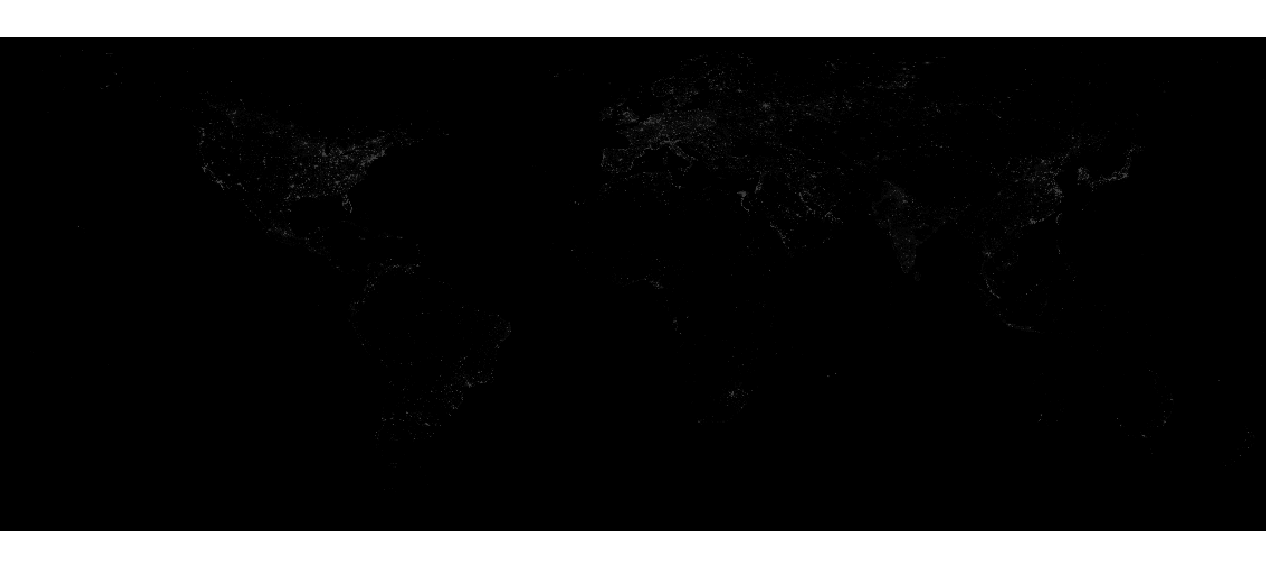
\includegraphics[width=1\linewidth]{figures/stable_full} \caption{\label{result_plot} The Raw Stable Lights Image}\label{fig:stable}
\end{figure}

\hypertarget{night-light-data-and-noise}{%
\section{\texorpdfstring{Night Light data and Noise
\label{problem}}{Night Light data and Noise }}\label{night-light-data-and-noise}}

\hypertarget{stable-lights-and-economic-activity}{%
\subsection{Stable Lights and Economic
Activity}\label{stable-lights-and-economic-activity}}

The Stable Lights Product is a

The most prominent difficulty, however, relates to the amount of noise
in the lower end of the light distribution due in part to the blooming
effect mentioned above. Standard practice using the stable lights data
set is to discard these values from analysis, thereby removing a large
proportion of cell observations.

Common solution to the problem of noise is to either filter out data
below a certain threshold, or set those values to 0.1 (Source NB NB NB)

\begin{figure}[H]
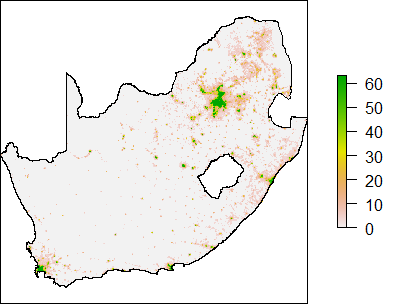
\includegraphics[width=0.5\linewidth]{figures/stable_SA} 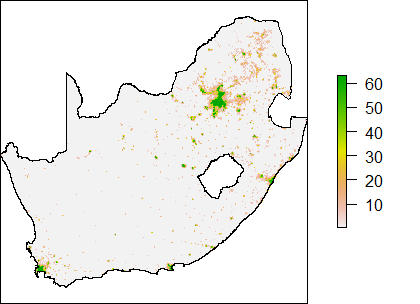
\includegraphics[width=0.5\linewidth]{figures/stable_SA_noise_filtered} \caption{\label{result_plot} Left - Raw Stable Lights; Right - Noise Discarded}\label{fig:stable_no_noise}
\end{figure}

\begin{figure}[H]
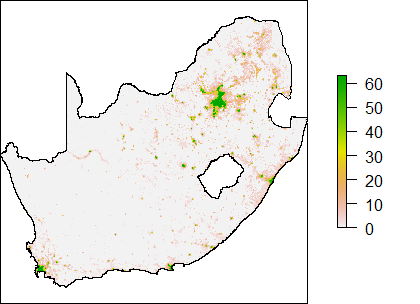
\includegraphics[width=1\linewidth]{figures/final} \caption{\label{result_plot} Human Lights Image }\label{fig:final}
\end{figure}

\hypertarget{method-and-data}{%
\section{\texorpdfstring{Method and Data
\label{Methodology}}{Method and Data }}\label{method-and-data}}

\begin{itemize}
\tightlist
\item
  Short overview of Määttä \& Lessmann
  (\protect\hyperlink{ref-maatta}{2019})
\end{itemize}

The filtering process used by Määttä \& Lessmann
(\protect\hyperlink{ref-maatta}{2019}) attempts to more accurately
detect \emph{human-generated} night light luminosity.

\hypertarget{data}{%
\subsection{Data}\label{data}}

Table \ref{variable_table} below gives an overview of the most important
variables used as inputs in the machine learning algorithm. The Global
Human Settlement Layer (GHSL) \emph{built-up} grid - satellite-derived
images of the world based on Landsat satellites - is used to classify
whether a certain area is more likely to contain human generated
light.\footnote{For more on the GHSL methodology, consult Pesaresi,
  Ehrlich, Ferri, Florczyk, Freire, Halkia, Julea, Kemper, Soille,
  Syrris \& others (\protect\hyperlink{ref-pesaresi2016operating}{2016})}.
The second and third variables constitute the two primary DMSP-OLS
products released by NOAA, and is also the most crucial inputs in the
filtering methodology. This is due to the fact that the subsequent
variables are derived from them. The \emph{local noise} variable is used
to identify those areas where background noise is systematically larger
than some threshold, and consists out of the number of pixels in a
window of 499 by 499 pixels below this threshold.\footnote{We follow
  Määttä \& Lessmann (\protect\hyperlink{ref-maatta}{2019}) in choosing
  the upper bound threshold value of 6 so as to be most strict in what
  is considered noise} The \emph{local detections} counts the number of
pixels where zero light is detected in a 399 by 399 window around a
pixel. The rest of the variables are generated to be regional input
variables that more closely describe the characteristics of luminosity
surrounding a specific pixel. By varying the size of the area around a
pixel, one more accurately accounts for spatial correlations in light
that is human generated.

\begin{table}
\begin{center}
\begin{tabular}{ |l|l|l| }
 \hline
 Input & Source & Description  \\ 
 \hline
  built up & GHSL & Landsat satellite images of built-up areas \\ 
  avg light & DMSP-OLS & average light per pixel over a year \\ 
  freq light & DMSP-OLS & proportion of days where light is detected per pixel \\
  local noise & Derived from DMSP-OLS & number of pixels below threshold in avg light image \\
  local detections & Derived from DMSP-OLS & accounts for regional differences in freq light \\
  lm freq 5 & Derived from DMSP-OLS & average of freq light in a 5 by 5 pixel area \\
  lm avg 25 & Derived from DMSP-OLS & average of avg light in a 25 by 25 pixel area \\
  lm freq 99 & Derived from DMSP-OLS & average of freq light in a 99 by 99 pixel area \\
  lm avg 199 & Derived from DMSP-OLS & average of avg light in a 199 by 199 pixel area \\
  \hline
\end{tabular}
\caption{Data Inputs}
\label{variable_table}
\end{center}
\end{table}

\hypertarget{methodology}{%
\subsection{Methodology}\label{methodology}}

The variables above constitute the primary inputs for Määttä \& Lessmann
(\protect\hyperlink{ref-maatta}{2019})`s 'Human Lights' product.
Methodologically, the following five steps are necessitated:

First, the regional night light variables are created from the original
\emph{avg light} and \emph{freq light} DMSP-OLS products.

Second, the world map is divided in various sub-regions, in preparation
that the random forest algorithm be run on each sub-region separately.
All the variable images are cropped into 2000-pixel square sub-regions,
which equates to about 3.4 million \(km^2\). Each sub-region consists of
approximately 4 million rows, whilst the model is trained on a 10\%
subsample.

\begin{longtable}[]{@{}l@{}}
\toprule
\endhead
5. Local Human Lights Process \\
However, the changes in the classification rule across the
sub-regions \\
causes a problem at their borders. The shifts in predicted
probabilities, and consequently the number \\
of lit pixels, are visibly clear. \\
The solution for smoothing the border effects is to move the sub-region
window in smaller steps \\
and then average the results. The step size should be as small as
possible, but we rapidly run into \\
computational constraints. Therefore, we decide to move the window in
steps of 250 pixels so that we \\
receive 64 values for each pixel. Unlike in the global approach, we now
set the number of lit pixels \\
within each window by using a 4\% tolerance level. This means that we
keep classifying light in pixels \\
as human-generated in the order of highest probability until 4\% of
avg\_light pixels with values below 5 \\
are included. By setting the amount of light with this tolerance
threshold, we avoid having to make \\
subjective choices of light amounts across regions or base them on the
built-up data. However, we have \\
to include a backstop or we end up adding lit pixels also in areas where
there is no human-generated \\
light at all. Therefore, we additionally set all pixels with a predicted
probability less than 20\% of being \\
human-generated to zero. \\
As described above, we classify light in each pixel 64 times by the
overlapping sub-region windows \\
as human-generated or not. After Step 3 in the filtering process, we
mosaic all the windows and \\
count the classifications. We then create the final product in Step 4 by
taking the light value from the \\
average visible band image if a pixel is classified as human-generated
more than eight times out of \\
64. Otherwise, we set the light value in a pixel to zero. The
requirement of eight human-generated \\
light classifications makes a final global adjustment to the amount of
light. We have chosen the light \\
amount settings in a way that balances the improvement in detecting
human-generated light while \\
keeping misclassifications at a low level. Howeve \\
\bottomrule
\end{longtable}

Many of the tasks needed for successful implementation of the filtering
procedure are intensive both in terms of computation and memory usage.
Due to computational limitations, we therefore employed AWS' EC2 cloud
computing platform for parallel computation. This proved costly,
however, and implementation thereby required some deviations from the
methodology presented in Määttä \& Lessmann
(\protect\hyperlink{ref-maatta}{2019}). Most crucially, the random
forest algorithm was only applied to a subset of the world data. As our
research interests entailed a specific country, South Africa, we limited
the regional sub-windows to a one-square window, roughly the size of
South Africa. Although this step may carry some costs in that it means
that less regional variability is accounted for, these costs are
mitigated by the possibility that there would not be large regional
variability within a single country in any case.

Other Differences:

\begin{itemize}
\tightlist
\item
  Size of area
\item
  Jitter size
\item
  Probability of human-generated
\item
  only f152001, we do f142001 and f182011 as well
\end{itemize}

\hypertarget{results}{%
\section{\texorpdfstring{Results
\label{Results}}{Results }}\label{results}}

\begin{itemize}
\tightlist
\item
  maps comparing stable lights with noise removed vs human-generated
  light (overlay map)
\item
  also amount/percentage of pixels saved
\item
  accuracy measures?
\end{itemize}

\hypertarget{discussion}{%
\section{\texorpdfstring{Discussion
\label{Discussion}}{Discussion }}\label{discussion}}

This paper extended the usage of a filtering methodology proposed by
Määttä \& Lessmann (\protect\hyperlink{ref-maatta}{2019}) with which to
separate background noise from human-generated nightlight data.

Our results echo those by Määttä \& Lessmann
(\protect\hyperlink{ref-maatta}{2019}): the RF algorithm introduces
great improvements in classification accuracy and thus greater accuracy
in filtering out background noise from the `Stable Lights' product. This
allows the researcher to do away with the need for quick-and-easy type
fixes to noisy data at the lower end of the luminosity distribution.

However, it is important to note what this method does not achieve. For
instance, the `Human Lights' product does not address the issue of
blooming or oversaturation at the high end of the luminosity spectrum.
Likewise, its spatial resolution remains low in comparison to more
modern products such as the Visible Infrared Imaging Radiometer Suite
(VIIRS), and it is recommended to use these products rather than the
DMSP-OLS `Stable Lights' or `Human Lights' products if possible.

\newpage

\hypertarget{references}{%
\section*{References}\label{references}}
\addcontentsline{toc}{section}{References}

\hypertarget{refs}{}
\begin{CSLReferences}{1}{0}
\leavevmode\vadjust pre{\hypertarget{ref-chen2011}{}}%
Chen, X. \& Nordhaus, W.D. 2011. Using luminosity data as a proxy for
economic statistics. \emph{Proceedings of the National Academy of
Sciences}. 108(21):8589--8594.

\leavevmode\vadjust pre{\hypertarget{ref-elvidge1997}{}}%
Elvidge, C.D., Baugh, K.E., Kihn, E.A., Kroehl, H.W., Davis, E.R. \&
Davis, C.W. 1997. Relation between satellite observed visible-near
infrared emissions, population, economic activity and electric power
consumption. \emph{International Journal of Remote Sensing}.
18(6):1373--1379.

\leavevmode\vadjust pre{\hypertarget{ref-henderson2012}{}}%
Henderson, J.V., Storeygard, A. \& Weil, D.N. 2012. Measuring economic
growth from outer space. \emph{American economic review}.
102(2):994--1028.

\leavevmode\vadjust pre{\hypertarget{ref-ivan2020nlinequality}{}}%
Ivan, K., Holobâcă, I.-H., Benedek, J. \& Török, I. 2020. Potential of
night-time lights to measure regional inequality. \emph{Remote Sensing}.
12(1):33.

\leavevmode\vadjust pre{\hypertarget{ref-maatta}{}}%
Määttä, I. \& Lessmann, C. 2019. Human lights. \emph{Remote Sensing}.
11(19):2194.

\leavevmode\vadjust pre{\hypertarget{ref-mellander2015night}{}}%
Mellander, C., Lobo, J., Stolarick, K. \& Matheson, Z. 2015. Night-time
light data: A good proxy measure for economic activity? \emph{PloS one}.
10(10):e0139779.

\leavevmode\vadjust pre{\hypertarget{ref-mveyange2015}{}}%
Mveyange, A. 2015. \emph{Night lights and regional income inequality in
africa}. WIDER Working Paper.

\leavevmode\vadjust pre{\hypertarget{ref-pesaresi2016operating}{}}%
Pesaresi, M., Ehrlich, D., Ferri, S., Florczyk, A., Freire, S., Halkia,
M., Julea, A., Kemper, T., et al. 2016. Operating procedure for the
production of the global human settlement layer from landsat data of the
epochs 1975, 1990, 2000, and 2014. \emph{Publications Office of the
European Union}. 1--62.

\end{CSLReferences}

\newpage

\hypertarget{appendix}{%
\section*{Appendix}\label{appendix}}
\addcontentsline{toc}{section}{Appendix}

\begin{itemize}
\tightlist
\item
  images of all the different local images - refer them back to
  variables table
\end{itemize}

\begin{figure}[H]
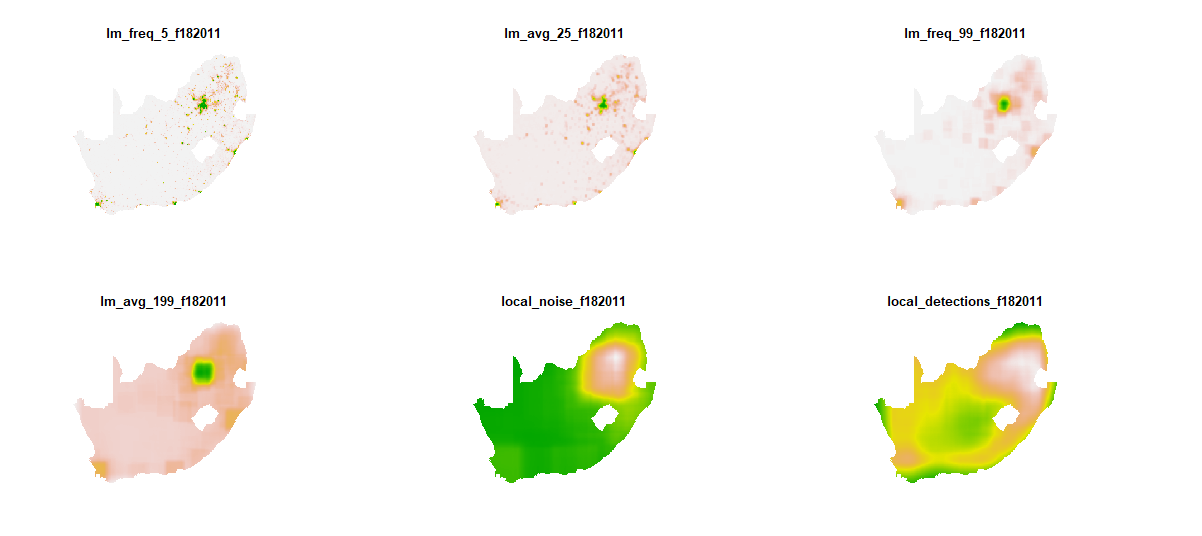
\includegraphics[width=1\linewidth]{figures/local_inputs} \caption{\label{local_images} Local Image Inputs}\label{fig:local_images}
\end{figure}

overlay plot of the above two with different colours

\bibliography{Tex/ref}





\end{document}
